\documentclass[letterpaper, 12pt]{article}
\usepackage{tabularx} 
\usepackage{amsmath} 
\usepackage{graphicx} 
\usepackage{caption}
\captionsetup[figure]{font=footnotesize}
\usepackage[margin=1.1in,letterpaper]{geometry}
\usepackage{cite} 
\usepackage{textcomp}
\usepackage[final]{hyperref} 
\hypersetup{
	colorlinks=true,      
	linkcolor=blue,        
	citecolor=blue,        
	filecolor=magenta,     
	urlcolor=blue         
}
\usepackage{blindtext}



\begin{document}
	
	\title{CMLS Homework 1 - Audio Event Classification}
	\author{E. Castelli, E. Intagliata, A. Rizzitiello, G. Zanocco}
	\date{April 2021}
	\maketitle
	
	\section{GitHub Repository}
	\url{https://github.com/ElisaCastelli/CMLS-HW1-Group11.git}
	
	\section{Introduction}
	The goal of the first CMLS homework which has been assigned to our group is to build a classifier that could predict the audio event recorded in an audio excerpt. As specified in the guidelines, all the experiments have been carried out using the \textit{UrbanSound8k}\footnote{UrbanSound8k dataset available at \url{https://urbansounddataset.weebly.com/urbansound8k.html}} sampled sounds collection. This database includes 8732 labeled audio excerpts of urban sounds organized in ten different categories, drawn from the urban sound taxonomy discussed in this paper \cite{sal14}. As suggested by the authors, we proceeded to work using the \textit{10-fold cross-validation} technique to evaluate our predictive model.
	
	
	\section{Data analysis}
	The samples of the dataset have been recorded from 10 classes of different sound sources: air conditioner, car horn, children playing, dog bark, drilling, engine idling, gun shot, jackhammer, siren and street music. The first thing we have done is a preprocessing analysis of the data, we have collected from the dataset, to understand which were the best characteristics to distinguish them and to check if the dataset is well balanced.
	
	We noticed that the classes “gun shot” and “car horn” have a few samples less than the other ones and that the great part of audio files have a duration of 4.0 seconds. Despite these small differences between audio and classes, as suggested from the authors of the dataset, we have decided to not modify the dataset and also to not do any reshuffling because the files have already been pre-sorted in a proper way to help the comparison.
	
	In order to manage easily the different audios, we have read the .csv file included in the dataset building for each row an object Sound and collect then in a list we have called soundList. In this way, we have retrieve all the information contained in the file and stored them into the attributes of Sound objects.
	
	In addition to the attribute already stored in the .csv file, we have chosen to add an array attribute in the object Sound to store the features we have computed for each sound during the reading. 
	\\
	
	We have tried different approaches but we have decided to choose as features the following ones:
	
	-	MFCC mean and standard deviation (25 coefficients each)
	
	-	Chroma features mean and standard deviation (12 coefficient each)
	
	-	Spectral contrast mean and standard deviation (4 coefficient each)
	\\
	
	In this way we have built a feature vector of 82 coefficient to capture different qualities about the audio over time, without exceeding in expensive computation.
	
	As suggested by the author of the dataset, we performed the 10-fold cross validation to do the training, test steps and the classification. Only at the end we have taken the ten different results and we have made an average on them.
	
	\section{Classification}
	Once the desired features were computed, we could proceed with the classification. We decided to use SVM (Support Vector Machine) as model for the classifier and RBF (radial basis function) as kernel function.

As for the training and testing steps, we proceeded as follows. At each iteration of the cross-validation algorihm we initialized a new model, then trained it on supervised data from 9 of the 10 predefined folds and finally tested it by predicting the labels of the samples contained in the remaining fold. The results of each prediction were stored for the evaluation part while the model was discarded.

The actual implementation of the SVM classifier is the one provided by the sklearn library. According to its documentation, this classifier is able to perform multiclass labeling using a one-vs-one scheme. This means that for every sample in the test set there is a set of multiple classifiers, one for each pair of possible classes which the sample can belong to. At the end of the prediction, the sample is assigned to the class that has received the most votes.

	\section{Results}
	In order to evaluate the performances of the algorithm, we evaluated the classification accuracy and the confusion matrix. 
Dealing with a multiclass classification problem, we used the \textit{sklearn} function \texttt{accuracy\_score} to compute the accuracy at each iteration. It returns the fraction of correctly classified samples:

\begin{equation}
[0.630, 0.646, 0.6086486486486486, 0.606, 0.703, 0.579, 0.663, 0.700, 0.680, 0.708]
\end{equation}
	
	 This gives us an average accuracy of about \textbf{ 65.2 \% } which is slightly below the results obtained in \cite{sal14}.
	
	The confusion matrix in \ref{fig:cm} is obtained by summing the confusion matrices obtained at each iteration.
	

\begin{figure}
  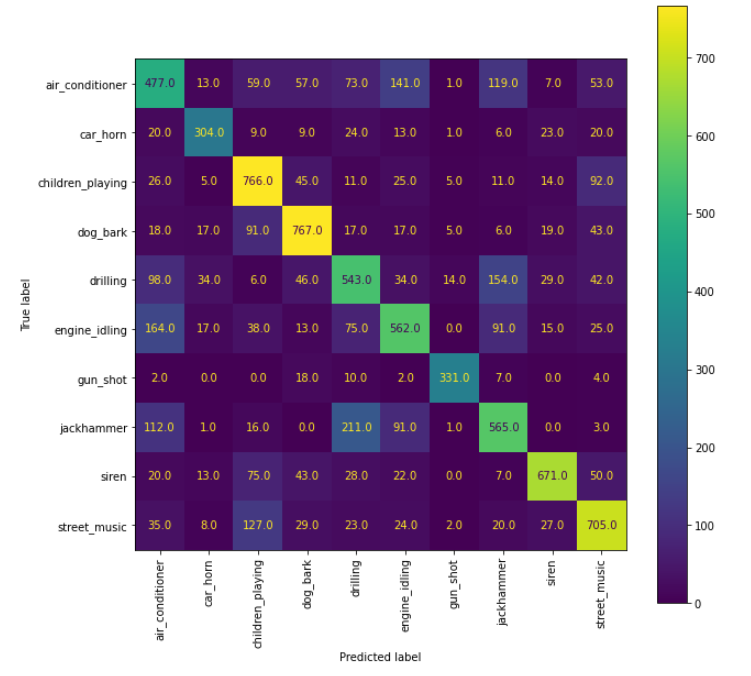
\includegraphics[width=\linewidth]{cm.png}
  \caption{Confusion Matrix}
  \label{fig:cm}
\end{figure}
	
We can see the performance between classes is in line with \cite{sal14}, too.
In particular both classifier, even relating on a different feature space, confuse pairs of classeswith similar timbres. FOr example: air conditioners and idling engines, jackhammers and drills, children and street music.
	
	
	\begin{thebibliography}{99}
		
		%1
		\bibitem{sal14}
		Justin Salamon, Christopher Jacoby, Juan Pablo Bello. A Dataset and Taxonomy for Urban Sound Research. \textit{Proceedings of the 22nd ACM international conference on Multimedia. November 2014, pages 1041–1044}. Cited at page \hyperlink{page.1}{1}.
		
		
	\end{thebibliography}

	
	
\end{document}
